% 1977 年云南卷第 3 题：两圆 O1、O2 外切于 C，外公切线 PQ 切两圆于 A、B，
% 过 C 的内公切线交 PQ 于 D，连接 AC、BC（按源卷第 2 页布局）
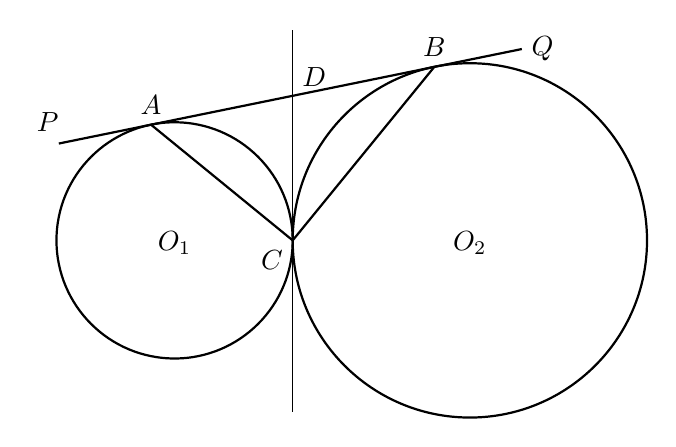
\begin{tikzpicture}[scale=1.5]
  \draw[thick] (0,0) circle (1);
  \draw[thick] (2.5,0) circle (1.5);
  \draw[thick] (-0.98,0.82)--(2.94,1.62);
  \draw[thin] (1,1.78)--(1,-1.45);
  \draw[thick] (-0.2,0.98)--(1,0);
  \draw[thick] (2.2,1.47)--(1,0);
  \node[above left] at (-0.9,0.84) {$P$};
  \node[above] at (-0.2,0.98) {$A$};
  \node[above right] at (1,1.22) {$D$};
  \node[above] at (2.2,1.47) {$B$};
  \node[right] at (2.94,1.62) {$Q$};
  \node at (0,-0.02) {$O_1$};
  \node at (2.5,-0.02) {$O_2$};
  \node[below left] at (1,0) {$C$};
\end{tikzpicture}
